\section{Trích xuất thực thể và quan hệ để xây dựng Knowledge Graph}
Để nâng cao khả năng suy luận logic trong hệ thống trả lời câu hỏi, chúng tôi chuyển đổi dữ liệu văn bản phi cấu trúc thành Knowledge Graph. KG là một cấu trúc dữ liệu dạng đồ thị, trong đó các nodes đại diện cho entities và các edges đại diện cho relationships giữa chúng. Việc xây dựng KG tự động từ văn bản lịch sử yêu cầu hai giai đoạn chính: trích xuất Entity và trích xuất Relationship.

\subsection{Trích xuất Entity}

Thực thể lịch sử được định nghĩa là các đối tượng có tên riêng hoặc định danh cụ thể, đóng vai trò là các nút trong đồ thị tri thức. Quy trình trích xuất sử dụng mô hình ngôn ngữ lớn \textbf{Deepseek-chat} làm hạt nhân xử lý, kết hợp với các bước tiền xử lý và hậu xử lý chuyên biệt cho từng chủ đề trong  SGK.

\vspace{0.5em}
\noindent\textbf{Định nghĩa Schema Entity chuẩn.}
Việc định nghĩa trước các Entity Types hợp lệ là bước quan trọng để đảm bảo tính nhất quán và khả năng truy vấn của KG. Dựa trên phân tích đặc thù của văn bản lịch sử sách giáo khoa, xác định được 11 Entity Types:

\begin{itemize}
    \item \textit{Nhân Vật}: Các cá nhân lịch sử có tên riêng (ví dụ: Hồ Chí Minh, Võ Nguyên Giáp). Đây là loại thực thể quan trọng vì nhân vật xuất hiện trong nhiều các sự kiện lịch sử.
    \item \textit{Tổ chức}: Các tổ chức, đảng phái, liên minh chính trị (ví dụ: Việt Minh, Liên hợp quốc). Việc phân biệt Tổ chức với Quốc gia giúp mô hình hóa chính xác vai trò của các thực thể trong các sự kiện.
    \item \textit{Quốc gia}: Các quốc gia, vùng lãnh thổ có chủ quyền. Phân loại này cần thiết vì quan hệ ngoại giao và xung đột thường diễn ra ở cấp độ quốc gia.
    \item \textit{Sự kiện}: Các sự kiện lịch sử quan trọng có tính chất mốc thời gian. Đây là loại thực thể đóng vai trò kết nối các nhân vật, tổ chức, và địa điểm.
    \item \textit{Chiến dịch/Trận đánh}: Các chiến dịch quân sự, chiến tranh. Việc tách riêng loại này khỏi Sự kiện chung giúp truy vấn chính xác hơn các câu hỏi về lịch sử quân sự.
    \item \textit{Hội nghị}: Các hội nghị quốc tế, đại hội quan trọng. Hội nghị thường là nơi ký kết các văn kiện, hiệp định, cần được mô hình hóa riêng.
    \item \textit{Văn kiện/Hiệp định}: Các văn bản pháp lý, hiệp định có tính ràng buộc. Đây là sản phẩm của các sự kiện và hội nghị, đồng thời là căn cứ cho các quyết định sau đó.
    \item \textit{Địa điểm}: Các địa danh lịch sử. Địa điểm giúp định vị không gian cho các sự kiện và chiến dịch.
    \item \textit{Chiến lược/Chủ trương}: Các đường lối, chính sách lớn. Loại này đặc biệt quan trọng trong lịch sử Việt Nam hiện đại với các chủ trương như Đổi mới.
    \item \textit{Khái niệm}: Các thuật ngữ, khái niệm lịch sử trừu tượng (ví dụ: Trật tự hai cực, Chiến tranh lạnh).
    \item \textit{Công trình}: Các công trình kiến trúc, di tích được xuất hiện.
\end{itemize}

\vspace{0.5em}
\noindent\textbf{Quy trình trích xuất thực thể.}
Pipeline xử lý được thiết kế theo nguyên tắc module hóa, cho phép tùy chỉnh linh hoạt cho từng chủ đề lịch sử:

\begin{enumerate}
    \item \textbf{Phân đoạn văn bản theo cửa sổ:} Văn bản được chia thành các cửa sổ không chồng lên nhau, mỗi cửa sổ chứa các câu liên tiếp. Kích thước này được chọn dựa trên thực nghiệm để đảm bảo: (a) đủ ngữ cảnh để mô hình nhận diện thực thể, (b) không quá dài gây nhiễu thông tin, và (c) phù hợp với giới hạn token của API. Mỗi cửa sổ được gắn metadata về vị trí bào gồm chỉ số câu bắt đầu/kết thúc và nguồn gốc là chủ đề, bài học để phục vụ việc truy xuất sau này.

    \item \textbf{Tạo prompt động theo chủ đề:} Thay vì sử dụng một prompt cố định, hệ thống tự động điều chỉnh prompt dựa trên chủ đề của văn bản đang xử lý. Lý do: mỗi chủ đề lịch sử có đặc thù riêng về loại thực thể ưu tiên, từ viết tắt chuyên ngành, và các nhân vật/tổ chức quan trọng. Ví dụ, với chủ đề ASEAN, prompt sẽ nhấn mạnh việc nhận diện các tổ chức quốc tế và các quốc gia thành viên; với chủ đề Hồ Chí Minh, prompt sẽ hướng dẫn mô hình nhận diện các tên gọi khác nhau của cùng một nhân vật (Nguyễn Ái Quốc, Văn Ba, Hồ Chí Minh). Prompt cũng được mở rộng các từ viết tắt (ví dụ: WTO $\rightarrow$ Tổ chức Thương mại Thế giới) để tăng khả năng nhận diện.

    \item \textbf{Gọi API và phân tích phản hồi:} Mỗi cửa sổ văn bản được gửi tới mô hình deepseek-chat kèm theo prompt đã tùy chỉnh. Phản hồi JSON từ mô hình được phân tích để trích xuất danh sách thực thể thô. Hệ thống theo dõi chi tiết từng request theo các chỉ số thời gian, số thực thể, trạng thái phục vụ việc giám sát và gỡ lỗi.

    \item \textbf{Lọc thực thể nhiễu:} Các thực thể trích xuất được đưa qua bộ lọc để loại bỏ nhiễu. Các trường hợp bị loại bỏ bao gồm: (a) thực thể quá chung chung không mang tính định danh (ví dụ: "chính phủ", "quân đội", "nhân dân"); (b) thực thể chỉ là ngày tháng đơn thuần không gắn với sự kiện cụ thể (ví dụ: "1945", "ngày 30"); (c) thực thể có độ dài quá ngắn (dưới 2 ký tự); (d) các từ mang tính cảm xúc, đánh giá (ví dụ: "vĩ đại", "thiêng liêng"). Việc lọc này giúp giảm nhiễu và tăng chất lượng của KG cuối cùng.

    \item \textbf{Phát hiện và gộp thực thể trùng lặp:} Vì các thực thể có thể xuất hiện ở nhiều cửa sổ với các biến thể tên gọi khác nhau, hệ thống sử dụng thuật toán so sánh chuỗi với ngưỡng tương đồng để phát hiện trùng lặp. Đặc biệt, với các thực thể dễ nhầm lẫn (như "Chiến tranh thế giới thứ nhất" và "Chiến tranh thế giới thứ hai"), hệ thống có logic riêng để phân tích số thứ tự và tránh gộp sai. Khi phát hiện trùng lặp, hệ thống gộp danh sách labels, tổng hợp các vị trí xuất hiện trong văn bản original\_text, và cập nhật số lần xuất hiện occurrence\_count.

    \item \textbf{Làm giàu thông tin theo chủ đề:} Sau khi trích xuất, các thực thể được bổ sung thông tin cấu trúc đặc thù theo chủ đề. Ví dụ: với các tên gọi của Hồ Chí Minh, hệ thống tự động gắn thông tin về thời kỳ sử dụng (Nguyễn Ái Quốc: 1919-1942); với các thành viên gia đình, gắn quan hệ họ hàng; với các tổ chức do Bác sáng lập, gắn năm thành lập và vai trò. Việc làm giàu này giúp KG chứa nhiều thông tin ngữ nghĩa hơn mà không cần trích xuất thêm từ văn bản.

    \item \textbf{Xử lý hậu kỳ và xuất kết quả:} Bước cuối cùng bao gồm làm sạch ID và labels chủ yếu là chuẩn hóa, loại bỏ các lần xuất hiện trùng lặp trong original\_text, và đơn giản hóa metadata. Kết quả được xuất ra file JSON với cấu trúc chuẩn hóa, sẵn sàng cho giai đoạn trích xuất quan hệ.
\end{enumerate}

% Component Diagram cho Entity Extraction Pipeline
% Sử dụng trong LaTeX với % Component Diagram cho Entity Extraction Pipeline
% Sử dụng trong LaTeX với % Component Diagram cho Entity Extraction Pipeline
% Sử dụng trong LaTeX với % Component Diagram cho Entity Extraction Pipeline
% Sử dụng trong LaTeX với \input{architecture_diagram.tex}

\begin{figure}[H]
\centering
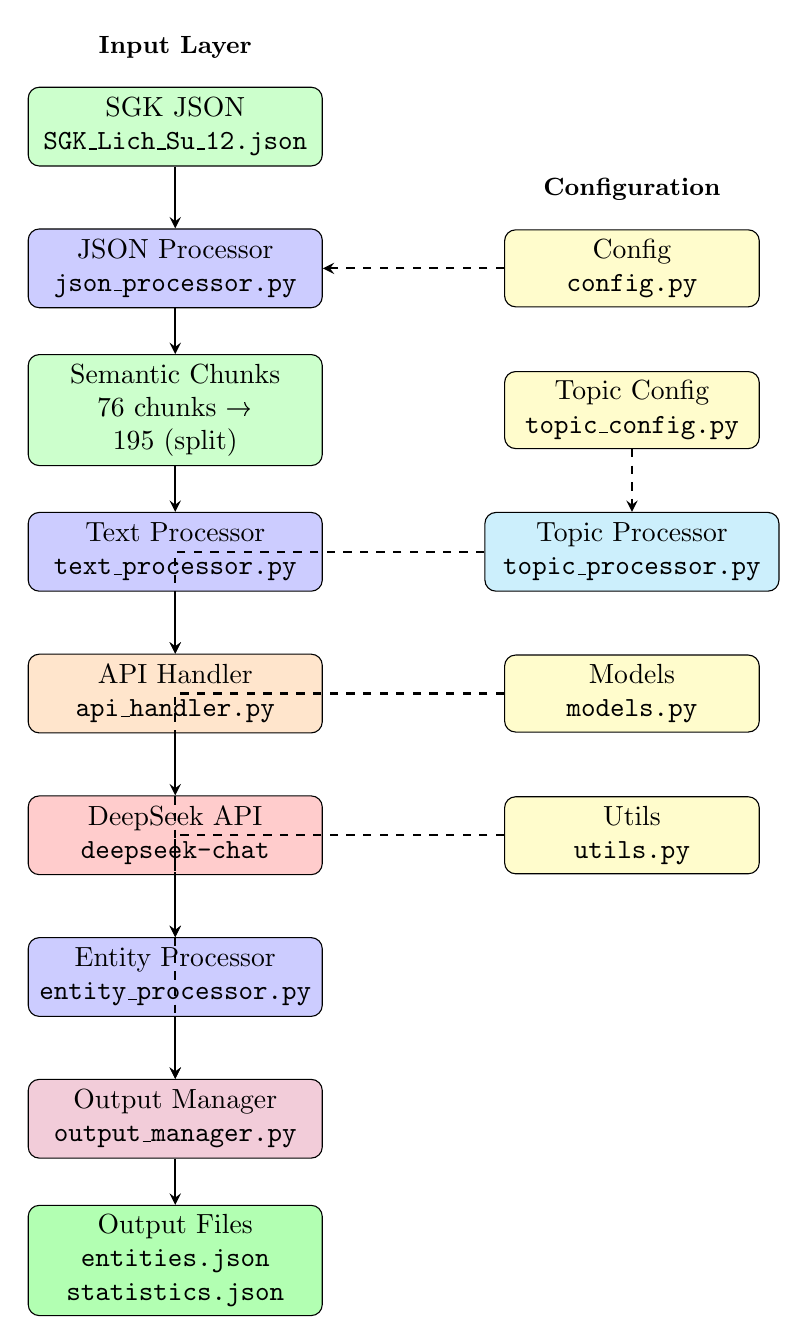
\begin{tikzpicture}[node distance=1.8cm, auto]
    % Styles
    \tikzstyle{datablock} = [rectangle, draw, fill=green!20, 
        text width=3.5cm, text centered, rounded corners, minimum height=1cm]
    \tikzstyle{component} = [rectangle, draw, fill=blue!20, 
        text width=3.5cm, text centered, rounded corners, minimum height=1cm]
    \tikzstyle{apiblock} = [rectangle, draw, fill=orange!20, 
        text width=3.5cm, text centered, rounded corners, minimum height=1cm]
    \tikzstyle{configblock} = [rectangle, draw, fill=yellow!20, 
        text width=3cm, text centered, rounded corners, minimum height=0.8cm]
    \tikzstyle{outputblock} = [rectangle, draw, fill=purple!20, 
        text width=3.5cm, text centered, rounded corners, minimum height=1cm]
    \tikzstyle{arrow} = [thick,->,>=stealth]
    \tikzstyle{dashedarrow} = [thick,->,>=stealth,dashed]
    
    % === LEFT COLUMN: Main Pipeline ===
    % Input Data
    \node [datablock] (input) {SGK JSON\\\texttt{SGK\_Lich\_Su\_12.json}};
    
    % JSON Processor
    \node [component, below of=input] (jsonproc) {JSON Processor\\\texttt{json\_processor.py}};
    
    % Semantic Chunks
    \node [datablock, below of=jsonproc] (chunks) {Semantic Chunks\\76 chunks → 195 (split)};
    
    % Text Processor
    \node [component, below of=chunks] (textproc) {Text Processor\\\texttt{text\_processor.py}};
    
    % API Handler
    \node [apiblock, below of=textproc] (apihandler) {API Handler\\\texttt{api\_handler.py}};
    
    % DeepSeek API (external)
    \node [apiblock, below of=apihandler, fill=red!20] (deepseek) {DeepSeek API\\\texttt{deepseek-chat}};
    
    % Entity Processor
    \node [component, below of=deepseek] (entityproc) {Entity Processor\\\texttt{entity\_processor.py}};
    
    % Output Manager
    \node [outputblock, below of=entityproc] (output) {Output Manager\\\texttt{output\_manager.py}};
    
    % Output Files
    \node [datablock, below of=output, fill=green!30] (outputfiles) {Output Files\\\texttt{entities.json}\\\texttt{statistics.json}};
    
    % === RIGHT COLUMN: Configuration & Support ===
    % Config
    \node [configblock, right of=jsonproc, xshift=4cm] (config) {Config\\\texttt{config.py}};
    
    % Topic Config Manager
    \node [configblock, below of=config] (topicconfig) {Topic Config\\\texttt{topic\_config.py}};
    
    % Topic Processor
    \node [component, below of=topicconfig, fill=cyan!20] (topicproc) {Topic Processor\\\texttt{topic\_processor.py}};
    
    % Models
    \node [configblock, below of=topicproc] (models) {Models\\\texttt{models.py}};
    
    % Utils
    \node [configblock, below of=models] (utils) {Utils\\\texttt{utils.py}};
    
    % === ARROWS: Main Flow ===
    \draw [arrow] (input) -- (jsonproc);
    \draw [arrow] (jsonproc) -- (chunks);
    \draw [arrow] (chunks) -- (textproc);
    \draw [arrow] (textproc) -- (apihandler);
    \draw [arrow] (apihandler) -- (deepseek);
    \draw [arrow] (deepseek) -- (entityproc);
    \draw [arrow] (entityproc) -- (output);
    \draw [arrow] (output) -- (outputfiles);
    
    % === ARROWS: Dependencies ===
    \draw [dashedarrow] (config) -- (jsonproc);
    \draw [dashedarrow] (topicconfig) -- (topicproc);
    \draw [dashedarrow] (topicproc) -| (apihandler);
    \draw [dashedarrow] (models) -| (entityproc);
    \draw [dashedarrow] (utils) -| (output);
    
    % === Labels ===
    \node [above of=input, yshift=-0.8cm, font=\small\bfseries] {Input Layer};
    \node [above of=config, yshift=-0.8cm, font=\small\bfseries] {Configuration};
    
\end{tikzpicture}
\caption{Kiến trúc tổng quan hệ thống Entity Extraction}
\label{fig:extract-architecture}
\end{figure}


\begin{figure}[H]
\centering
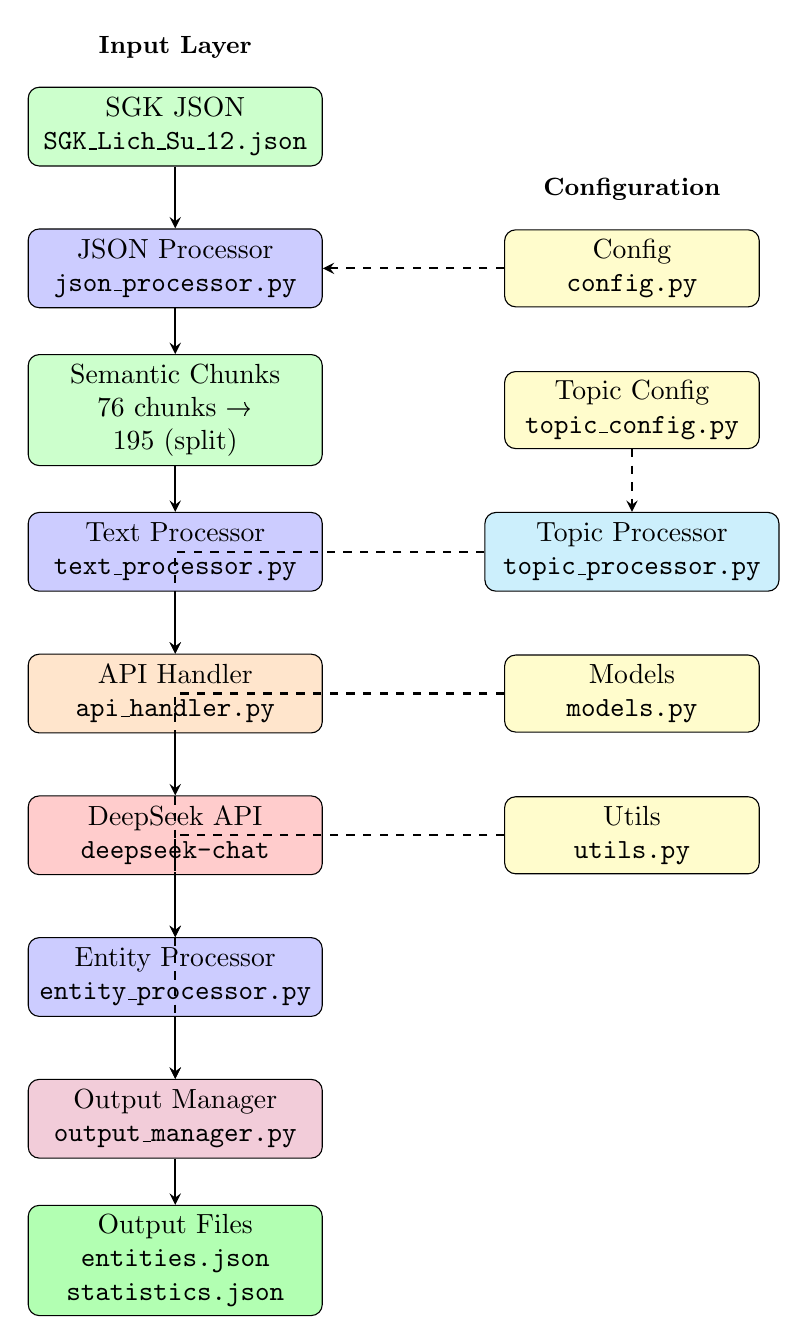
\begin{tikzpicture}[node distance=1.8cm, auto]
    % Styles
    \tikzstyle{datablock} = [rectangle, draw, fill=green!20, 
        text width=3.5cm, text centered, rounded corners, minimum height=1cm]
    \tikzstyle{component} = [rectangle, draw, fill=blue!20, 
        text width=3.5cm, text centered, rounded corners, minimum height=1cm]
    \tikzstyle{apiblock} = [rectangle, draw, fill=orange!20, 
        text width=3.5cm, text centered, rounded corners, minimum height=1cm]
    \tikzstyle{configblock} = [rectangle, draw, fill=yellow!20, 
        text width=3cm, text centered, rounded corners, minimum height=0.8cm]
    \tikzstyle{outputblock} = [rectangle, draw, fill=purple!20, 
        text width=3.5cm, text centered, rounded corners, minimum height=1cm]
    \tikzstyle{arrow} = [thick,->,>=stealth]
    \tikzstyle{dashedarrow} = [thick,->,>=stealth,dashed]
    
    % === LEFT COLUMN: Main Pipeline ===
    % Input Data
    \node [datablock] (input) {SGK JSON\\\texttt{SGK\_Lich\_Su\_12.json}};
    
    % JSON Processor
    \node [component, below of=input] (jsonproc) {JSON Processor\\\texttt{json\_processor.py}};
    
    % Semantic Chunks
    \node [datablock, below of=jsonproc] (chunks) {Semantic Chunks\\76 chunks → 195 (split)};
    
    % Text Processor
    \node [component, below of=chunks] (textproc) {Text Processor\\\texttt{text\_processor.py}};
    
    % API Handler
    \node [apiblock, below of=textproc] (apihandler) {API Handler\\\texttt{api\_handler.py}};
    
    % DeepSeek API (external)
    \node [apiblock, below of=apihandler, fill=red!20] (deepseek) {DeepSeek API\\\texttt{deepseek-chat}};
    
    % Entity Processor
    \node [component, below of=deepseek] (entityproc) {Entity Processor\\\texttt{entity\_processor.py}};
    
    % Output Manager
    \node [outputblock, below of=entityproc] (output) {Output Manager\\\texttt{output\_manager.py}};
    
    % Output Files
    \node [datablock, below of=output, fill=green!30] (outputfiles) {Output Files\\\texttt{entities.json}\\\texttt{statistics.json}};
    
    % === RIGHT COLUMN: Configuration & Support ===
    % Config
    \node [configblock, right of=jsonproc, xshift=4cm] (config) {Config\\\texttt{config.py}};
    
    % Topic Config Manager
    \node [configblock, below of=config] (topicconfig) {Topic Config\\\texttt{topic\_config.py}};
    
    % Topic Processor
    \node [component, below of=topicconfig, fill=cyan!20] (topicproc) {Topic Processor\\\texttt{topic\_processor.py}};
    
    % Models
    \node [configblock, below of=topicproc] (models) {Models\\\texttt{models.py}};
    
    % Utils
    \node [configblock, below of=models] (utils) {Utils\\\texttt{utils.py}};
    
    % === ARROWS: Main Flow ===
    \draw [arrow] (input) -- (jsonproc);
    \draw [arrow] (jsonproc) -- (chunks);
    \draw [arrow] (chunks) -- (textproc);
    \draw [arrow] (textproc) -- (apihandler);
    \draw [arrow] (apihandler) -- (deepseek);
    \draw [arrow] (deepseek) -- (entityproc);
    \draw [arrow] (entityproc) -- (output);
    \draw [arrow] (output) -- (outputfiles);
    
    % === ARROWS: Dependencies ===
    \draw [dashedarrow] (config) -- (jsonproc);
    \draw [dashedarrow] (topicconfig) -- (topicproc);
    \draw [dashedarrow] (topicproc) -| (apihandler);
    \draw [dashedarrow] (models) -| (entityproc);
    \draw [dashedarrow] (utils) -| (output);
    
    % === Labels ===
    \node [above of=input, yshift=-0.8cm, font=\small\bfseries] {Input Layer};
    \node [above of=config, yshift=-0.8cm, font=\small\bfseries] {Configuration};
    
\end{tikzpicture}
\caption{Kiến trúc tổng quan hệ thống Entity Extraction}
\label{fig:extract-architecture}
\end{figure}


\begin{figure}[H]
\centering
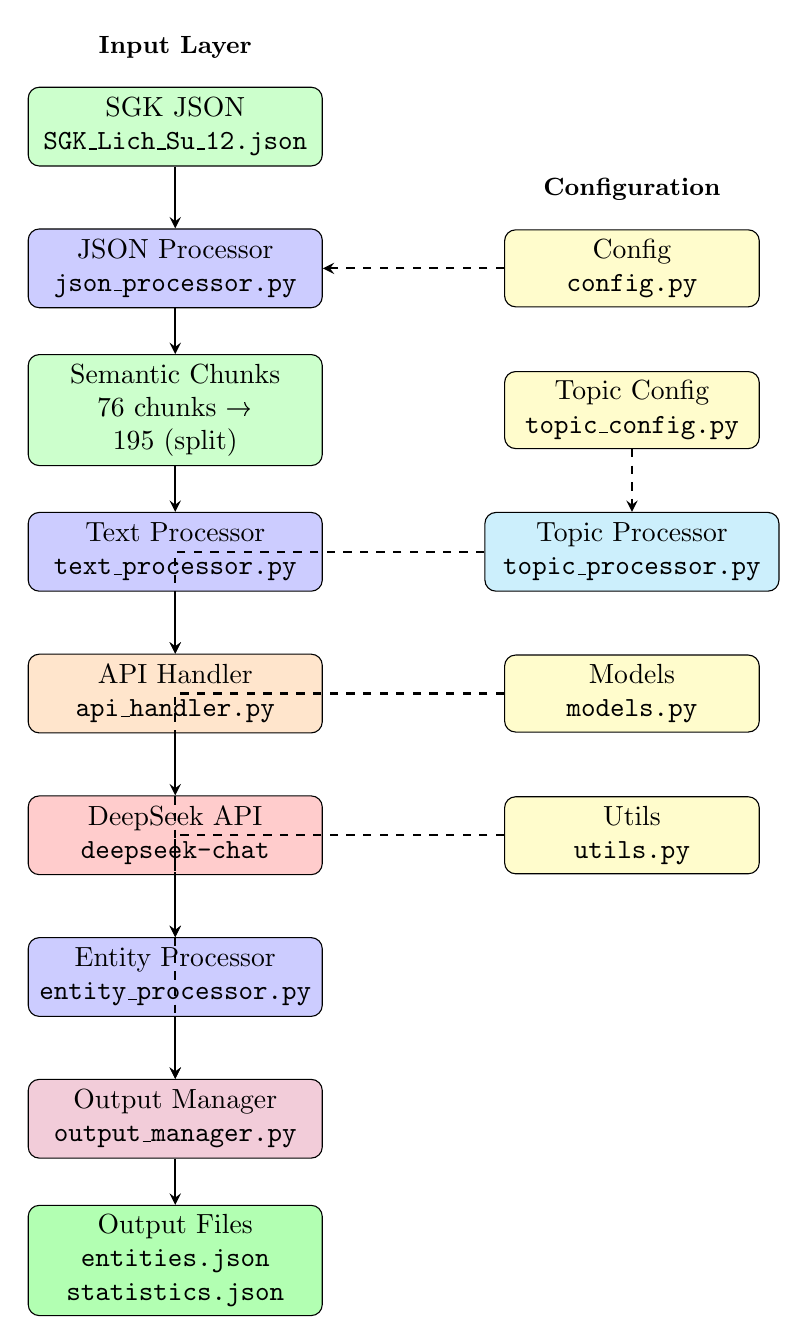
\begin{tikzpicture}[node distance=1.8cm, auto]
    % Styles
    \tikzstyle{datablock} = [rectangle, draw, fill=green!20, 
        text width=3.5cm, text centered, rounded corners, minimum height=1cm]
    \tikzstyle{component} = [rectangle, draw, fill=blue!20, 
        text width=3.5cm, text centered, rounded corners, minimum height=1cm]
    \tikzstyle{apiblock} = [rectangle, draw, fill=orange!20, 
        text width=3.5cm, text centered, rounded corners, minimum height=1cm]
    \tikzstyle{configblock} = [rectangle, draw, fill=yellow!20, 
        text width=3cm, text centered, rounded corners, minimum height=0.8cm]
    \tikzstyle{outputblock} = [rectangle, draw, fill=purple!20, 
        text width=3.5cm, text centered, rounded corners, minimum height=1cm]
    \tikzstyle{arrow} = [thick,->,>=stealth]
    \tikzstyle{dashedarrow} = [thick,->,>=stealth,dashed]
    
    % === LEFT COLUMN: Main Pipeline ===
    % Input Data
    \node [datablock] (input) {SGK JSON\\\texttt{SGK\_Lich\_Su\_12.json}};
    
    % JSON Processor
    \node [component, below of=input] (jsonproc) {JSON Processor\\\texttt{json\_processor.py}};
    
    % Semantic Chunks
    \node [datablock, below of=jsonproc] (chunks) {Semantic Chunks\\76 chunks → 195 (split)};
    
    % Text Processor
    \node [component, below of=chunks] (textproc) {Text Processor\\\texttt{text\_processor.py}};
    
    % API Handler
    \node [apiblock, below of=textproc] (apihandler) {API Handler\\\texttt{api\_handler.py}};
    
    % DeepSeek API (external)
    \node [apiblock, below of=apihandler, fill=red!20] (deepseek) {DeepSeek API\\\texttt{deepseek-chat}};
    
    % Entity Processor
    \node [component, below of=deepseek] (entityproc) {Entity Processor\\\texttt{entity\_processor.py}};
    
    % Output Manager
    \node [outputblock, below of=entityproc] (output) {Output Manager\\\texttt{output\_manager.py}};
    
    % Output Files
    \node [datablock, below of=output, fill=green!30] (outputfiles) {Output Files\\\texttt{entities.json}\\\texttt{statistics.json}};
    
    % === RIGHT COLUMN: Configuration & Support ===
    % Config
    \node [configblock, right of=jsonproc, xshift=4cm] (config) {Config\\\texttt{config.py}};
    
    % Topic Config Manager
    \node [configblock, below of=config] (topicconfig) {Topic Config\\\texttt{topic\_config.py}};
    
    % Topic Processor
    \node [component, below of=topicconfig, fill=cyan!20] (topicproc) {Topic Processor\\\texttt{topic\_processor.py}};
    
    % Models
    \node [configblock, below of=topicproc] (models) {Models\\\texttt{models.py}};
    
    % Utils
    \node [configblock, below of=models] (utils) {Utils\\\texttt{utils.py}};
    
    % === ARROWS: Main Flow ===
    \draw [arrow] (input) -- (jsonproc);
    \draw [arrow] (jsonproc) -- (chunks);
    \draw [arrow] (chunks) -- (textproc);
    \draw [arrow] (textproc) -- (apihandler);
    \draw [arrow] (apihandler) -- (deepseek);
    \draw [arrow] (deepseek) -- (entityproc);
    \draw [arrow] (entityproc) -- (output);
    \draw [arrow] (output) -- (outputfiles);
    
    % === ARROWS: Dependencies ===
    \draw [dashedarrow] (config) -- (jsonproc);
    \draw [dashedarrow] (topicconfig) -- (topicproc);
    \draw [dashedarrow] (topicproc) -| (apihandler);
    \draw [dashedarrow] (models) -| (entityproc);
    \draw [dashedarrow] (utils) -| (output);
    
    % === Labels ===
    \node [above of=input, yshift=-0.8cm, font=\small\bfseries] {Input Layer};
    \node [above of=config, yshift=-0.8cm, font=\small\bfseries] {Configuration};
    
\end{tikzpicture}
\caption{Kiến trúc tổng quan hệ thống Entity Extraction}
\label{fig:extract-architecture}
\end{figure}


\begin{figure}[H]
\centering
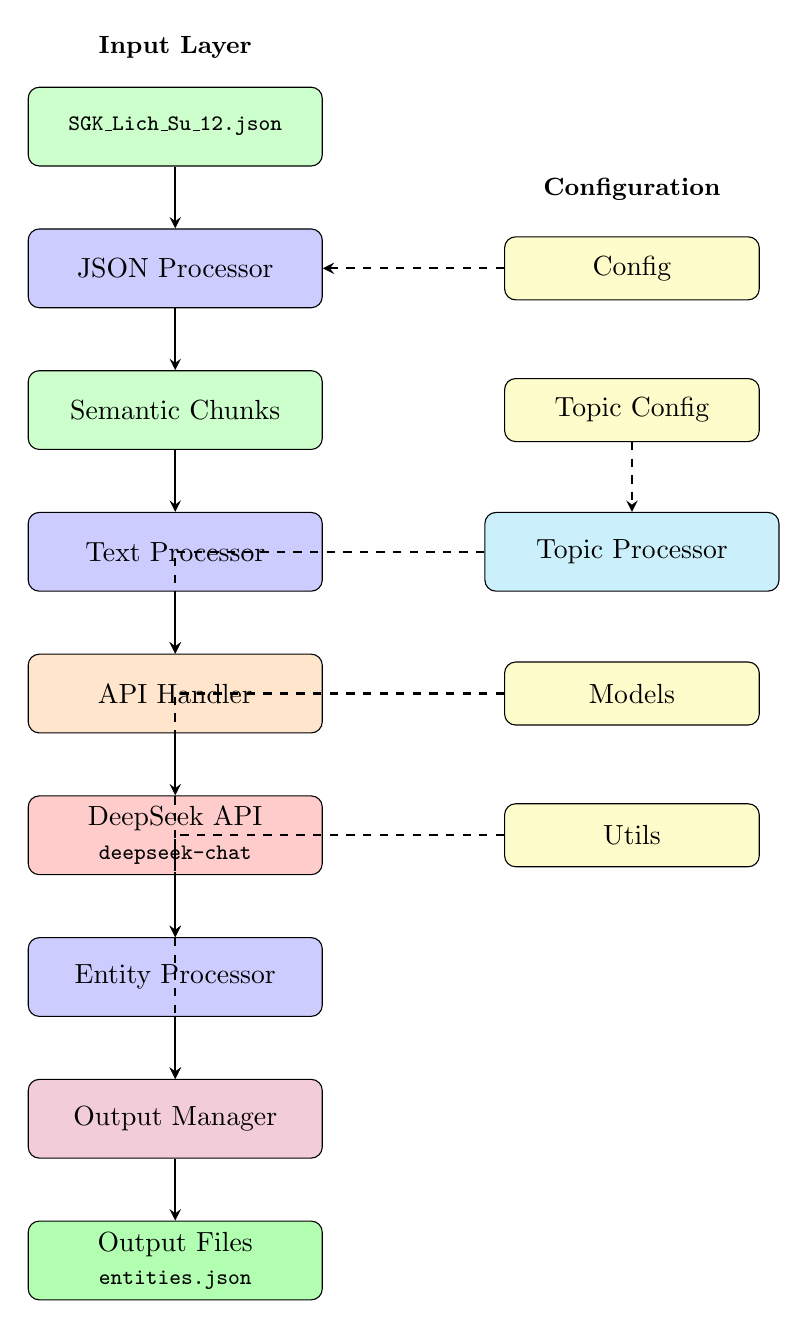
\begin{tikzpicture}[node distance=1.8cm, auto]
    % Styles
    \tikzstyle{datablock} = [rectangle, draw, fill=green!20, 
        text width=3.5cm, text centered, rounded corners, minimum height=1cm]
    \tikzstyle{component} = [rectangle, draw, fill=blue!20, 
        text width=3.5cm, text centered, rounded corners, minimum height=1cm]
    \tikzstyle{apiblock} = [rectangle, draw, fill=orange!20, 
        text width=3.5cm, text centered, rounded corners, minimum height=1cm]
    \tikzstyle{configblock} = [rectangle, draw, fill=yellow!20, 
        text width=3cm, text centered, rounded corners, minimum height=0.8cm]
    \tikzstyle{outputblock} = [rectangle, draw, fill=purple!20, 
        text width=3.5cm, text centered, rounded corners, minimum height=1cm]
    \tikzstyle{arrow} = [thick,->,>=stealth]
    \tikzstyle{dashedarrow} = [thick,->,>=stealth,dashed]
    
    % === LEFT COLUMN: Main Pipeline ===
    % Input Data
    \node [datablock] (input) {{\footnotesize\texttt{SGK\_Lich\_Su\_12.json}}};
    
    % JSON Processor
    \node [component, below of=input] (jsonproc) {JSON Processor};
    
    % Semantic Chunks
    \node [datablock, below of=jsonproc] (chunks) {Semantic Chunks};
    
    % Text Processor
    \node [component, below of=chunks] (textproc) {Text Processor};
    
    % API Handler
    \node [apiblock, below of=textproc] (apihandler) {API Handler};
    
    % DeepSeek API (external)
    \node [apiblock, below of=apihandler, fill=red!20] (deepseek) {DeepSeek API\\{\footnotesize\texttt{deepseek-chat}}};
    
    % Entity Processor
    \node [component, below of=deepseek] (entityproc) {Entity Processor};
    
    % Output Manager
    \node [outputblock, below of=entityproc] (output) {Output Manager};
    
    % Output Files
    \node [datablock, below of=output, fill=green!30] (outputfiles) {Output Files\\{\footnotesize\texttt{entities.json}}};
    
    % === RIGHT COLUMN: Configuration & Support ===
    % Config
    \node [configblock, right of=jsonproc, xshift=4cm] (config) {Config};
    
    % Topic Config Manager
    \node [configblock, below of=config] (topicconfig) {Topic Config};
    
    % Topic Processor
    \node [component, below of=topicconfig, fill=cyan!20] (topicproc) {Topic Processor};
    
    % Models
    \node [configblock, below of=topicproc] (models) {Models};
    
    % Utils
    \node [configblock, below of=models] (utils) {Utils};
    
    % === ARROWS: Main Flow ===
    \draw [arrow] (input) -- (jsonproc);
    \draw [arrow] (jsonproc) -- (chunks);
    \draw [arrow] (chunks) -- (textproc);
    \draw [arrow] (textproc) -- (apihandler);
    \draw [arrow] (apihandler) -- (deepseek);
    \draw [arrow] (deepseek) -- (entityproc);
    \draw [arrow] (entityproc) -- (output);
    \draw [arrow] (output) -- (outputfiles);
    
    % === ARROWS: Dependencies ===
    \draw [dashedarrow] (config) -- (jsonproc);
    \draw [dashedarrow] (topicconfig) -- (topicproc);
    \draw [dashedarrow] (topicproc) -| (apihandler);
    \draw [dashedarrow] (models) -| (entityproc);
    \draw [dashedarrow] (utils) -| (output);
    
    % === Labels ===
    \node [above of=input, yshift=-0.8cm, font=\small\bfseries] {Input Layer};
    \node [above of=config, yshift=-0.8cm, font=\small\bfseries] {Configuration};
    
\end{tikzpicture}
\caption{Kiến trúc tổng quan hệ thống Entity Extraction}
\label{fig:extract-architecture}
\end{figure}


\vspace{0.5em}
\noindent\textbf{Cấu trúc dữ liệu thực thể.}
Mỗi thực thể trong file kết quả chứa các trường: 
\texttt{id} (định danh duy nhất bằng tiếng Việt), 
\texttt{label} (danh sách các tên gọi/bí danh), 
\texttt{type} (loại thực thể theo schema đã định nghĩa), 
\texttt{description} (mô tả ngắn gọn), 
\texttt{original\_text} (danh sách các lần xuất hiện kèm thông tin chủ đề, bài học, và đoạn văn chính xác), 
\texttt{properties} (các thuộc tính cấu trúc như năm thành lập, vai trò), \texttt{metadata} (thông tin bổ sung về timeline), 
\texttt{confidence} (điểm tin cậy), và 
\texttt{occurrence\_count} (tổng số lần xuất hiện trong corpus).


\subsection{Trích xuất Relationship}
\label{subsec:relationship_extraction}

Sau khi có danh sách thực thể, bước tiếp theo là xác định các mối quan hệ ngữ nghĩa giữa chúng. Quan hệ trong KG được biểu diễn dưới dạng bộ ba (triplet): \texttt{(Subject, Predicate, Object)}, trong đó Subject và Object là các thực thể, còn Predicate mô tả mối quan hệ giữa chúng. Chất lượng của các quan hệ quyết định trực tiếp khả năng suy luận đa bước của hệ thống.

\vspace{0.5em}
\noindent\textbf{Nguyên tắc thiết kế pipeline.}
Quy trình trích xuất quan hệ được thiết kế dựa trên các nguyên tắc sau:

\begin{itemize}
    \item \textbf{Context-aware Extraction:} Thay vì trích xuất quan hệ từ toàn bộ văn bản, hệ thống tập trung vào các cửa sổ ngữ cảnh chứa ít nhất 2 thực thể đã được nhận diện. Lý do: quan hệ có ý nghĩa thường xuất hiện khi các thực thể được đề cập gần nhau trong các đoạn văn bản.
    
    \item \textbf{Entity-centric Prompting:} Prompt được sinh động dựa trên thực thể mục tiêu đang xét, cung cấp cho mô hình thông tin về loại thực thể, các tên gọi, và gợi ý các loại quan hệ phù hợp. Điều này giúp mô hình tập trung và tăng độ chính xác.
    
    \item \textbf{Multi-phase Processing:} Pipeline hoạt động theo 3 giai đoạn để đảm bảo độ bao phủ tối đa: xử lý chính theo chủ đề, bổ sung cho thực thể chưa kết nối, và kết nối theo nhóm chủ đề.
\end{itemize}

\vspace{0.5em}
\noindent\textbf{Quy trình trích xuất quan hệ.}

\begin{enumerate}
    \item \textbf{Nạp thực thể và tạo Entity Lookup:} Danh sách thực thể từ giai đoạn trước được nạp và tạo bảng tra cứu nhanh theo ID và các labels. Việc này cho phép xác thực tức thì xem một thực thể trong quan hệ có tồn tại trong danh sách đã tạo trước đó theo chủ đề tương ứng hay không.

    \item \textbf{Tạo cửa sổ trượt chồng lên nhau:} Khác với giai đoạn trích xuất thực thể sử dụng cửa sổ không chồng lên nhau, giai đoạn này sử dụng cửa sổ trượt chồng chập. Lý do: quan hệ có thể trải dài qua nhiều câu, việc chồng chập đảm bảo không bỏ sót các quan hệ nằm ở các câu liên tiếp.

    \item \textbf{Sinh prompt động theo thực thể mục tiêu:} Với mỗi cửa sổ, hệ thống sinh prompt động dựa trên thực thể trọng tâm đang xét. Prompt bao gồm: (a) thông tin chi tiết về thực thể mục tiêu (ID, Type, Labels, Description, số lần xuất hiện); (b) danh sách các loại quan hệ gợi ý phù hợp với loại thực thể (ví dụ: Nhân Vật $\rightarrow$ \{lãnh\_đạo, tham\_gia, thành\_lập, ký\_kết, chỉ\_huy\}; Tổ chức $\rightarrow$ \{thành\_lập, hợp\_tác, thuộc\_về, thành\_viên\_của\}); (c) danh sách các thực thể ứng viên có khả năng liên quan (ưu tiên các thực thể đồng xuất hiện trong cùng đoạn văn và có type tương thích); (d) ví dụ minh họa về định dạng quan hệ mong muốn.

    \item \textbf{Gọi API và trích xuất quan hệ thô:} Prompt hoàn chỉnh được gửi tới mô hình deepseek-chat. Phản hồi JSON chứa danh sách các quan hệ dạng \texttt{\{subject\_id, predicate, object\_id, evidence, confidence\}}. Hệ thống quản lý API key áp dụng cơ chế thử lại 3 lần khi gặp lỗi mạng.

    \item \textbf{Xác thực quan hệ:} Mỗi quan hệ trích xuất được đưa qua bộ lọc nghiêm ngặt:
    \begin{itemize}
        \item Subject và Object phải tồn tại trong Entity Lookup bằng cách tìm kiếm cả theo ID lẫn labels.
        \item Subject và Object không được trùng nhau để loại bỏ quan hệ phản xạ vô nghĩa.
        \item Predicate phải có độ dài tối thiểu 2 ký tự và mang ý nghĩa hành động cụ thể.
        \item Câu văn chứng minh phải có độ dài tối thiểu 8 ký tự và chứa ít nhất một trong hai thực thể hoặc các từ khóa liên kết.
    \end{itemize}
    Việc xác thực nghiêm ngặt giúp loại bỏ các quan hệ nhiễu do mô hình hallucination.

    \item \textbf{Gộp quan hệ trùng lặp:} Khi cùng một quan hệ (cùng Subject, Predicate, Object) được trích xuất từ nhiều cửa sổ khác nhau, hệ thống gộp chúng thành một bản ghi duy nhất: (a) tăng occurrence\_count để phản ánh tần suất xuất hiện (tần suất cao thường đồng nghĩa với độ tin cậy cao); (b) lưu trữ tất cả các câu văn chứng minh vào danh sách supporting\_sentences để hỗ trợ truy vết nguồn gốc; (c) cập nhật confidence bằng giá trị cao nhất trong các quan hệ trùng lặp.

    \item \textbf{Bổ sung quan hệ cho thực thể chưa kết nối:} Sau giai đoạn chính, hệ thống xác định các thực thể vẫn chưa có bất kỳ quan hệ nào . Với mỗi thực thể này, hệ thống tìm kiếm các cửa sổ ngữ cảnh chứa nó trong văn bản gốc và thực hiện trích xuất quan hệ có chủ đích với target\_entity\_id được chỉ định rõ ràng. Điều này buộc mô hình tập trung tìm kiếm quan hệ cho thực thể mục tiêu thay vì quét chung.

    \item \textbf{Kết nối theo nhóm chủ đề:} Giai đoạn cuối cùng nhằm tối đa hóa độ bao phủ của KG. Các thực thể vẫn chưa kết nối được nhóm theo loại, sau đó hệ thống tìm kiếm các file văn bản có chứa đồng thời nhiều thực thể cùng nhóm. Quan hệ được trích xuất từ các cửa sổ ngữ cảnh chung này với hy vọng phát hiện các liên kết gián tiếp giữa các thực thể cùng chủ đề.
\end{enumerate}

% Component Diagram cho Knowledge Graph (Relationship Extraction) Pipeline
% Sử dụng trong LaTeX với % Component Diagram cho Knowledge Graph (Relationship Extraction) Pipeline
% Sử dụng trong LaTeX với % Component Diagram cho Knowledge Graph (Relationship Extraction) Pipeline
% Sử dụng trong LaTeX với % Component Diagram cho Knowledge Graph (Relationship Extraction) Pipeline
% Sử dụng trong LaTeX với \input{architecture_kg_diagram.tex}

\begin{figure}[H]
\centering
\begin{tikzpicture}[node distance=1.8cm, auto]
    % Styles
    \tikzstyle{datablock} = [rectangle, draw, fill=green!20, 
        text width=3.5cm, text centered, rounded corners, minimum height=1cm]
    \tikzstyle{component} = [rectangle, draw, fill=blue!20, 
        text width=3.5cm, text centered, rounded corners, minimum height=1cm]
    \tikzstyle{apiblock} = [rectangle, draw, fill=orange!20, 
        text width=3.5cm, text centered, rounded corners, minimum height=1cm]
    \tikzstyle{configblock} = [rectangle, draw, fill=yellow!20, 
        text width=3cm, text centered, rounded corners, minimum height=0.8cm]
    \tikzstyle{outputblock} = [rectangle, draw, fill=purple!20, 
        text width=3.5cm, text centered, rounded corners, minimum height=1cm]
    \tikzstyle{arrow} = [thick,->,>=stealth]
    \tikzstyle{dashedarrow} = [thick,->,>=stealth,dashed]
    
    % === LEFT COLUMN: Main Pipeline ===
    % Input Data
    \node [datablock] (input) {SGK JSON\\+ Entities JSON};
    
    % JSON Processor
    \node [component, below of=input] (jsonproc) {JSON Processor};
    
    % Semantic Chunks
    \node [datablock, below of=jsonproc] (chunks) {Semantic Chunks\\(76 → 311 với overlap)};
    
    % Text Processor  
    \node [component, below of=chunks] (textproc) {Text Processor};
    
    % Relationship Processor
    \node [component, below of=textproc, fill=cyan!20] (relproc) {Relationship Processor};
    
    % API Handler
    \node [apiblock, below of=relproc] (apihandler) {API Handler};
    
    % DeepSeek API (external)
    \node [apiblock, below of=apihandler, fill=red!20] (deepseek) {DeepSeek API};
    
    % KG Builder
    \node [component, below of=deepseek] (kgbuilder) {KG Builder};
    
    % Output Manager
    \node [outputblock, below of=kgbuilder] (output) {Output Manager};
    
    % Output Files
    \node [datablock, below of=output, fill=green!30] (outputfiles) {Knowledge Graph\\(JSON)};
    
    % === RIGHT COLUMN: Configuration & Support ===
    % Config
    \node [configblock, right of=jsonproc, xshift=4cm] (config) {Config};
    
    % Entity Processor
    \node [configblock, below of=config] (entityproc) {Entity Processor};
    
    % Topic Config
    \node [configblock, below of=entityproc] (topicconfig) {Topic Config};
    
    % Topic Processor
    \node [component, below of=topicconfig, fill=cyan!20] (topicproc) {Topic Processor};
    
    % Models
    \node [configblock, below of=topicproc] (models) {Models\\(Entity, Triplet, KG)};
    
    % Utils
    \node [configblock, below of=models] (utils) {Utils};
    
    % === ARROWS: Main Flow ===
    \draw [arrow] (input) -- (jsonproc);
    \draw [arrow] (jsonproc) -- (chunks);
    \draw [arrow] (chunks) -- (textproc);
    \draw [arrow] (textproc) -- (relproc);
    \draw [arrow] (relproc) -- (apihandler);
    \draw [arrow] (apihandler) -- (deepseek);
    \draw [arrow] (deepseek) -- (kgbuilder);
    \draw [arrow] (kgbuilder) -- (output);
    \draw [arrow] (output) -- (outputfiles);
    
    % === ARROWS: Dependencies ===
    \draw [dashedarrow] (config) -- (jsonproc);
    \draw [dashedarrow] (entityproc) -| (relproc);
    \draw [dashedarrow] (topicconfig) -- (topicproc);
    \draw [dashedarrow] (topicproc) -| (apihandler);
    \draw [dashedarrow] (models) -| (kgbuilder);
    \draw [dashedarrow] (utils) -| (output);
    
    % === Labels ===
    \node [above of=input, yshift=-0.8cm, font=\small\bfseries] {Input Layer};
    \node [above of=config, yshift=-0.8cm, font=\small\bfseries] {Configuration};
    
\end{tikzpicture}
\caption{Kiến trúc tổng quan hệ thống Relationship Extraction}
\label{fig:extract-kg-architecture}
\end{figure}


\begin{figure}[H]
\centering
\begin{tikzpicture}[node distance=1.8cm, auto]
    % Styles
    \tikzstyle{datablock} = [rectangle, draw, fill=green!20, 
        text width=3.5cm, text centered, rounded corners, minimum height=1cm]
    \tikzstyle{component} = [rectangle, draw, fill=blue!20, 
        text width=3.5cm, text centered, rounded corners, minimum height=1cm]
    \tikzstyle{apiblock} = [rectangle, draw, fill=orange!20, 
        text width=3.5cm, text centered, rounded corners, minimum height=1cm]
    \tikzstyle{configblock} = [rectangle, draw, fill=yellow!20, 
        text width=3cm, text centered, rounded corners, minimum height=0.8cm]
    \tikzstyle{outputblock} = [rectangle, draw, fill=purple!20, 
        text width=3.5cm, text centered, rounded corners, minimum height=1cm]
    \tikzstyle{arrow} = [thick,->,>=stealth]
    \tikzstyle{dashedarrow} = [thick,->,>=stealth,dashed]
    
    % === LEFT COLUMN: Main Pipeline ===
    % Input Data
    \node [datablock] (input) {SGK JSON\\+ Entities JSON};
    
    % JSON Processor
    \node [component, below of=input] (jsonproc) {JSON Processor};
    
    % Semantic Chunks
    \node [datablock, below of=jsonproc] (chunks) {Semantic Chunks\\(76 → 311 với overlap)};
    
    % Text Processor  
    \node [component, below of=chunks] (textproc) {Text Processor};
    
    % Relationship Processor
    \node [component, below of=textproc, fill=cyan!20] (relproc) {Relationship Processor};
    
    % API Handler
    \node [apiblock, below of=relproc] (apihandler) {API Handler};
    
    % DeepSeek API (external)
    \node [apiblock, below of=apihandler, fill=red!20] (deepseek) {DeepSeek API};
    
    % KG Builder
    \node [component, below of=deepseek] (kgbuilder) {KG Builder};
    
    % Output Manager
    \node [outputblock, below of=kgbuilder] (output) {Output Manager};
    
    % Output Files
    \node [datablock, below of=output, fill=green!30] (outputfiles) {Knowledge Graph\\(JSON)};
    
    % === RIGHT COLUMN: Configuration & Support ===
    % Config
    \node [configblock, right of=jsonproc, xshift=4cm] (config) {Config};
    
    % Entity Processor
    \node [configblock, below of=config] (entityproc) {Entity Processor};
    
    % Topic Config
    \node [configblock, below of=entityproc] (topicconfig) {Topic Config};
    
    % Topic Processor
    \node [component, below of=topicconfig, fill=cyan!20] (topicproc) {Topic Processor};
    
    % Models
    \node [configblock, below of=topicproc] (models) {Models\\(Entity, Triplet, KG)};
    
    % Utils
    \node [configblock, below of=models] (utils) {Utils};
    
    % === ARROWS: Main Flow ===
    \draw [arrow] (input) -- (jsonproc);
    \draw [arrow] (jsonproc) -- (chunks);
    \draw [arrow] (chunks) -- (textproc);
    \draw [arrow] (textproc) -- (relproc);
    \draw [arrow] (relproc) -- (apihandler);
    \draw [arrow] (apihandler) -- (deepseek);
    \draw [arrow] (deepseek) -- (kgbuilder);
    \draw [arrow] (kgbuilder) -- (output);
    \draw [arrow] (output) -- (outputfiles);
    
    % === ARROWS: Dependencies ===
    \draw [dashedarrow] (config) -- (jsonproc);
    \draw [dashedarrow] (entityproc) -| (relproc);
    \draw [dashedarrow] (topicconfig) -- (topicproc);
    \draw [dashedarrow] (topicproc) -| (apihandler);
    \draw [dashedarrow] (models) -| (kgbuilder);
    \draw [dashedarrow] (utils) -| (output);
    
    % === Labels ===
    \node [above of=input, yshift=-0.8cm, font=\small\bfseries] {Input Layer};
    \node [above of=config, yshift=-0.8cm, font=\small\bfseries] {Configuration};
    
\end{tikzpicture}
\caption{Kiến trúc tổng quan hệ thống Relationship Extraction}
\label{fig:extract-kg-architecture}
\end{figure}


\begin{figure}[H]
\centering
\begin{tikzpicture}[node distance=1.8cm, auto]
    % Styles
    \tikzstyle{datablock} = [rectangle, draw, fill=green!20, 
        text width=3.5cm, text centered, rounded corners, minimum height=1cm]
    \tikzstyle{component} = [rectangle, draw, fill=blue!20, 
        text width=3.5cm, text centered, rounded corners, minimum height=1cm]
    \tikzstyle{apiblock} = [rectangle, draw, fill=orange!20, 
        text width=3.5cm, text centered, rounded corners, minimum height=1cm]
    \tikzstyle{configblock} = [rectangle, draw, fill=yellow!20, 
        text width=3cm, text centered, rounded corners, minimum height=0.8cm]
    \tikzstyle{outputblock} = [rectangle, draw, fill=purple!20, 
        text width=3.5cm, text centered, rounded corners, minimum height=1cm]
    \tikzstyle{arrow} = [thick,->,>=stealth]
    \tikzstyle{dashedarrow} = [thick,->,>=stealth,dashed]
    
    % === LEFT COLUMN: Main Pipeline ===
    % Input Data
    \node [datablock] (input) {SGK JSON\\+ Entities JSON};
    
    % JSON Processor
    \node [component, below of=input] (jsonproc) {JSON Processor};
    
    % Semantic Chunks
    \node [datablock, below of=jsonproc] (chunks) {Semantic Chunks\\(76 → 311 với overlap)};
    
    % Text Processor  
    \node [component, below of=chunks] (textproc) {Text Processor};
    
    % Relationship Processor
    \node [component, below of=textproc, fill=cyan!20] (relproc) {Relationship Processor};
    
    % API Handler
    \node [apiblock, below of=relproc] (apihandler) {API Handler};
    
    % DeepSeek API (external)
    \node [apiblock, below of=apihandler, fill=red!20] (deepseek) {DeepSeek API};
    
    % KG Builder
    \node [component, below of=deepseek] (kgbuilder) {KG Builder};
    
    % Output Manager
    \node [outputblock, below of=kgbuilder] (output) {Output Manager};
    
    % Output Files
    \node [datablock, below of=output, fill=green!30] (outputfiles) {Knowledge Graph\\(JSON)};
    
    % === RIGHT COLUMN: Configuration & Support ===
    % Config
    \node [configblock, right of=jsonproc, xshift=4cm] (config) {Config};
    
    % Entity Processor
    \node [configblock, below of=config] (entityproc) {Entity Processor};
    
    % Topic Config
    \node [configblock, below of=entityproc] (topicconfig) {Topic Config};
    
    % Topic Processor
    \node [component, below of=topicconfig, fill=cyan!20] (topicproc) {Topic Processor};
    
    % Models
    \node [configblock, below of=topicproc] (models) {Models\\(Entity, Triplet, KG)};
    
    % Utils
    \node [configblock, below of=models] (utils) {Utils};
    
    % === ARROWS: Main Flow ===
    \draw [arrow] (input) -- (jsonproc);
    \draw [arrow] (jsonproc) -- (chunks);
    \draw [arrow] (chunks) -- (textproc);
    \draw [arrow] (textproc) -- (relproc);
    \draw [arrow] (relproc) -- (apihandler);
    \draw [arrow] (apihandler) -- (deepseek);
    \draw [arrow] (deepseek) -- (kgbuilder);
    \draw [arrow] (kgbuilder) -- (output);
    \draw [arrow] (output) -- (outputfiles);
    
    % === ARROWS: Dependencies ===
    \draw [dashedarrow] (config) -- (jsonproc);
    \draw [dashedarrow] (entityproc) -| (relproc);
    \draw [dashedarrow] (topicconfig) -- (topicproc);
    \draw [dashedarrow] (topicproc) -| (apihandler);
    \draw [dashedarrow] (models) -| (kgbuilder);
    \draw [dashedarrow] (utils) -| (output);
    
    % === Labels ===
    \node [above of=input, yshift=-0.8cm, font=\small\bfseries] {Input Layer};
    \node [above of=config, yshift=-0.8cm, font=\small\bfseries] {Configuration};
    
\end{tikzpicture}
\caption{Kiến trúc tổng quan hệ thống Relationship Extraction}
\label{fig:extract-kg-architecture}
\end{figure}


\begin{figure}[H]
\centering
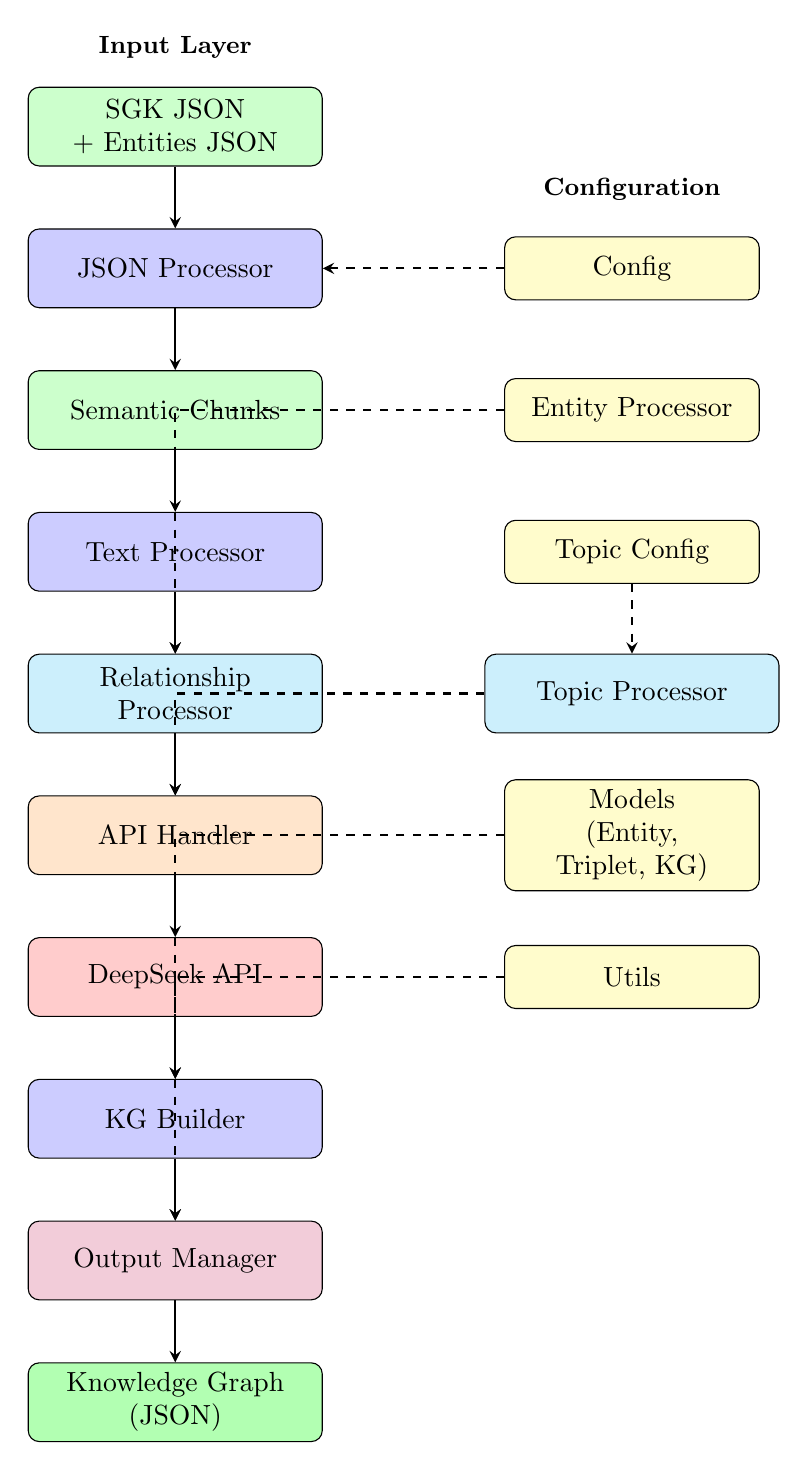
\begin{tikzpicture}[node distance=1.8cm, auto]
    % Styles
    \tikzstyle{datablock} = [rectangle, draw, fill=green!20, 
        text width=3.5cm, text centered, rounded corners, minimum height=1cm]
    \tikzstyle{component} = [rectangle, draw, fill=blue!20, 
        text width=3.5cm, text centered, rounded corners, minimum height=1cm]
    \tikzstyle{apiblock} = [rectangle, draw, fill=orange!20, 
        text width=3.5cm, text centered, rounded corners, minimum height=1cm]
    \tikzstyle{configblock} = [rectangle, draw, fill=yellow!20, 
        text width=3cm, text centered, rounded corners, minimum height=0.8cm]
    \tikzstyle{outputblock} = [rectangle, draw, fill=purple!20, 
        text width=3.5cm, text centered, rounded corners, minimum height=1cm]
    \tikzstyle{arrow} = [thick,->,>=stealth]
    \tikzstyle{dashedarrow} = [thick,->,>=stealth,dashed]
    
    % === LEFT COLUMN: Main Pipeline ===
    % Input Data
    \node [datablock] (input) {SGK JSON\\+ Entities JSON};
    
    % JSON Processor
    \node [component, below of=input] (jsonproc) {JSON Processor};
    
    % Semantic Chunks
    \node [datablock, below of=jsonproc] (chunks) {Semantic Chunks};
    
    % Text Processor  
    \node [component, below of=chunks] (textproc) {Text Processor};
    
    % Relationship Processor
    \node [component, below of=textproc, fill=cyan!20] (relproc) {Relationship Processor};
    
    % API Handler
    \node [apiblock, below of=relproc] (apihandler) {API Handler};
    
    % DeepSeek API (external)
    \node [apiblock, below of=apihandler, fill=red!20] (deepseek) {DeepSeek API};
    
    % KG Builder
    \node [component, below of=deepseek] (kgbuilder) {KG Builder};
    
    % Output Manager
    \node [outputblock, below of=kgbuilder] (output) {Output Manager};
    
    % Output Files
    \node [datablock, below of=output, fill=green!30] (outputfiles) {Knowledge Graph\\(JSON)};
    
    % === RIGHT COLUMN: Configuration & Support ===
    % Config
    \node [configblock, right of=jsonproc, xshift=4cm] (config) {Config};
    
    % Entity Processor
    \node [configblock, below of=config] (entityproc) {Entity Processor};
    
    % Topic Config
    \node [configblock, below of=entityproc] (topicconfig) {Topic Config};
    
    % Topic Processor
    \node [component, below of=topicconfig, fill=cyan!20] (topicproc) {Topic Processor};
    
    % Models
    \node [configblock, below of=topicproc] (models) {Models\\(Entity, Triplet, KG)};
    
    % Utils
    \node [configblock, below of=models] (utils) {Utils};
    
    % === ARROWS: Main Flow ===
    \draw [arrow] (input) -- (jsonproc);
    \draw [arrow] (jsonproc) -- (chunks);
    \draw [arrow] (chunks) -- (textproc);
    \draw [arrow] (textproc) -- (relproc);
    \draw [arrow] (relproc) -- (apihandler);
    \draw [arrow] (apihandler) -- (deepseek);
    \draw [arrow] (deepseek) -- (kgbuilder);
    \draw [arrow] (kgbuilder) -- (output);
    \draw [arrow] (output) -- (outputfiles);
    
    % === ARROWS: Dependencies ===
    \draw [dashedarrow] (config) -- (jsonproc);
    \draw [dashedarrow] (entityproc) -| (relproc);
    \draw [dashedarrow] (topicconfig) -- (topicproc);
    \draw [dashedarrow] (topicproc) -| (apihandler);
    \draw [dashedarrow] (models) -| (kgbuilder);
    \draw [dashedarrow] (utils) -| (output);
    
    % === Labels ===
    \node [above of=input, yshift=-0.8cm, font=\small\bfseries] {Input Layer};
    \node [above of=config, yshift=-0.8cm, font=\small\bfseries] {Configuration};
    
\end{tikzpicture}
\caption{Kiến trúc tổng quan hệ thống Relationship Extraction}
\label{fig:extract-kg-architecture}
\end{figure}

\vspace{0.5em}
\noindent\textbf{Cấu trúc dữ liệu Knowledge Graph.}
File kết quả chứa hai thành phần:
\begin{itemize}
    \item \texttt{entities}: Mảng các đối tượng Entity với đầy đủ thông tin như đã mô tả ở phần trích xuất thực thể.
    \item \texttt{triplets}: Mảng các bộ ba quan hệ, mỗi triplet chứa: \texttt{subject\_id} (ID thực thể nguồn), \texttt{predicate} (động từ/cụm động từ mô tả quan hệ bằng tiếng Việt), \texttt{object\_id} (ID thực thể đích), \texttt{confidence} (điểm tin cậy 0.0-1.0), \texttt{occurrence\_count} (số lần quan hệ được phát hiện), \texttt{supporting\_sentences} (danh sách các câu văn gốc chứng minh quan hệ kèm thông tin về nguồn gốc file), và \texttt{metadata} (thông tin về phương pháp trích xuất: gemini\_window\_analysis, supplemental\_context\_analysis, hoặc thematic\_group\_analysis).
\end{itemize}

\subsection{Tải dữ liệu Knowledge Graph lên Neo4j}

Sau khi hoàn thành việc trích xuất thực thể và quan hệ, Knowledge Graph được lưu trữ dưới dạng file JSON và cần được nạp vào cơ sở dữ liệu đồ thị Neo4j. Bước này là bước quan trọng để chuyển đổi tri thức đã được cấu trúc hóa thành một kho dữ liệu đồ thị có thể truy vấn trực tiếp, phục vụ cho giai đoạn truy xuất trong pipeline GraphRAG. Quy trình tải dữ liệu được thiết kế nhằm đảm bảo tính toàn vẹn dữ liệu, khả năng truy vấn hiệu quả và sự ổn định của hệ thống.

\paragraph{Chuẩn bị và Chuẩn hóa Dữ liệu}
Trước khi tiến hành nạp, dữ liệu đồ thị thô cần được tiền xử lý và chuẩn hóa để tương thích với các ràng buộc của Neo4j. Công việc này bao gồm:
\begin{itemize}
    \item \textbf{Làm sạch và Chuẩn hóa IDs:} Các ký tự đặc biệt không hợp lệ trong tên thực thể và định danh được loại bỏ hoặc thay thế, chỉ giữ lại các ký tự chữ cái bao gồm cả ký tự có dấu tiếng Việt, chữ số, dấu gạch dưới và gạch ngang. Điều này đảm bảo mọi định danh đều an toàn để sử dụng trong các truy vấn Cypher.
    \item \textbf{Chuẩn hóa Loại Quan hệ:} Các predicate được trích xuất từ triples phải được chuyển đổi thành định dạng phù hợp với quy ước đặt tên của Neo4j. Thông thường, chúng được chuyển thành dạng chữ in hoa với dấu gạch dưới (ví dụ: \texttt{LÃNH\_ĐẠO}, \texttt{DIỄN\_RA\_TẠI}).
\end{itemize}

\paragraph{Quy trình Nạp Entities và Relationships}
Dữ liệu sau khi chuẩn hóa được nạp vào Neo4j thông qua hai giai đoạn chính, sử dụng ngôn ngữ truy vấn Cypher:
\begin{enumerate}
    \item \textbf{Nạp Node Thực thể:} Mỗi thực thể trong KG được ánh xạ thành một node duy nhất trong Neo4j. Mỗi node được gán một hoặc nhiều labels dựa trên loại thực thể (ví dụ: \texttt{:Nhân Vật}, \texttt{:Sự Kiện}) và chứa các thuộc tính mô tả như (\texttt{label}), (\texttt{description}), (\texttt{id}) và liên kết đến văn bản nguồn (\texttt{source\_text}). Các thuộc tính có cấu trúc phức tạp được serialize thành chuỗi JSON trước khi lưu trữ.
    \item \textbf{Nạp Quan hệ dưới dạng Edges:} Các triplet (subject, predicate, object) được chuyển đổi thành các cạnh có hướng nối giữa các node. Quá trình này sử dụng câu lệnh \texttt{MATCH} để tìm node nguồn và node đích dựa trên định danh, sau đó tạo một quan hệ với loại (\texttt{type}) tương ứng với predicate. Các thuộc tính bổ sung của quan hệ cũng được lưu trữ ngay trên cạnh này.
\end{enumerate}

\paragraph{Triển khai và Đảm bảo Độ tin cậy}
Quy trình nạp được triển khai bằng một script tự động, tuân thủ các phương pháp tốt nhất để đảm bảo độ tin cậy:
\begin{itemize}
    \item \textbf{Kết nối và Khởi tạo:} Script thiết lập kết nối an toàn tới phiên bản Neo4j được triển khai trên cloud Neo4j Aura thông qua driver chính thức.
    \item \textbf{Làm sạch Môi trường:} Để tránh xung đột, toàn bộ dữ liệu đồ thị cũ có thể được xóa trước khi nạp bộ dữ liệu mới.
    \item \textbf{Batch Transactions:} Các thao tác tạo node và quan hệ được nhóm thành các transactions để tăng hiệu suất và đảm bảo atomicity. Nếu một phần của transactions thất bại, toàn bộ transactions sẽ được rollback để duy trì tính nhất quán của đồ thị.
    \item \textbf{Xử lý Ngoại lệ và Logging:} Cơ chế try-catch được áp dụng để xử lý các ngoại lệ có thể phát sinh (như định danh trùng lặp, vi phạm ràng buộc). Mọi lỗi đều được ghi lại chi tiết vào nhật ký, cho phép quá trình tiếp tục với các bản ghi hợp lệ khác và hỗ trợ việc gỡ lỗi sau này.
\end{itemize}

Kết quả của quy trình này là một cơ sở dữ liệu đồ thị Neo4j hoàn chỉnh, trong đó tri thức lịch sử đã được mã hóa thành một mạng lưới các nút và quan hệ có cấu trúc. Cơ sở dữ liệu này trở thành nền tảng cho việc thực thi các truy vấn đồ thị phức tạp sử dụng ngôn ngữ Cypher trong các bước truy xuất thông tin tiếp theo của hệ thống GraphRAG.